\subsubsection{Каскад с Общим Коллектрором}

\begin{center}
\begin{figure}[h!]
\center{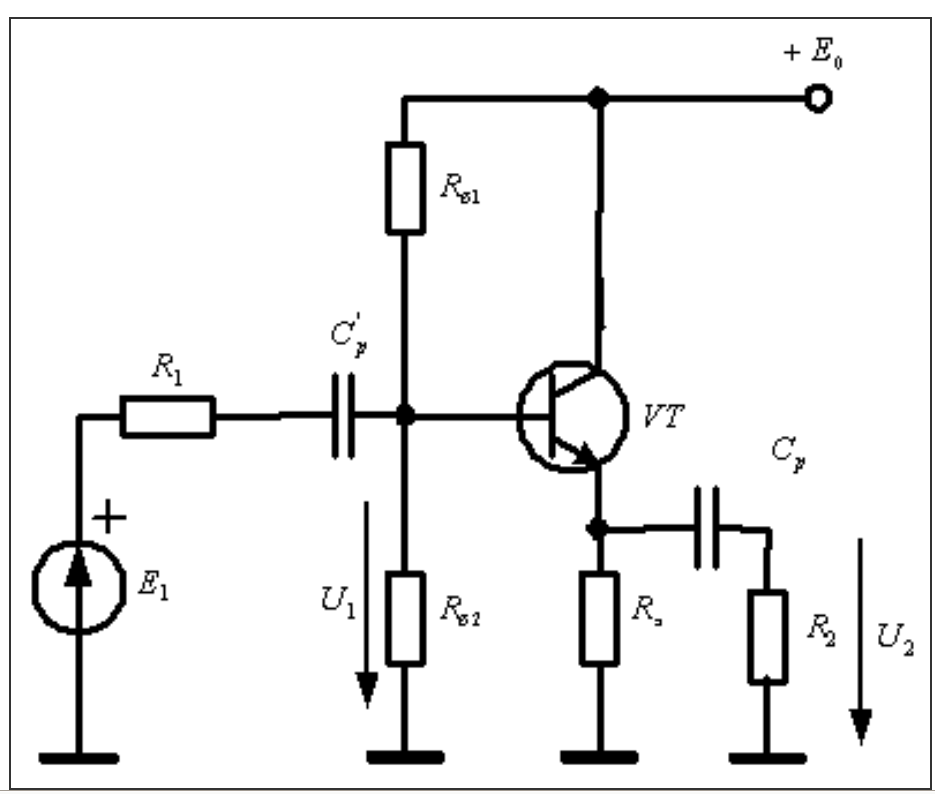
\includegraphics[scale=0.7]{OK.png}}
\caption{ОК}
\end{figure}
\end{center}

\begin{center}
\begin{figure}[h!]
\center{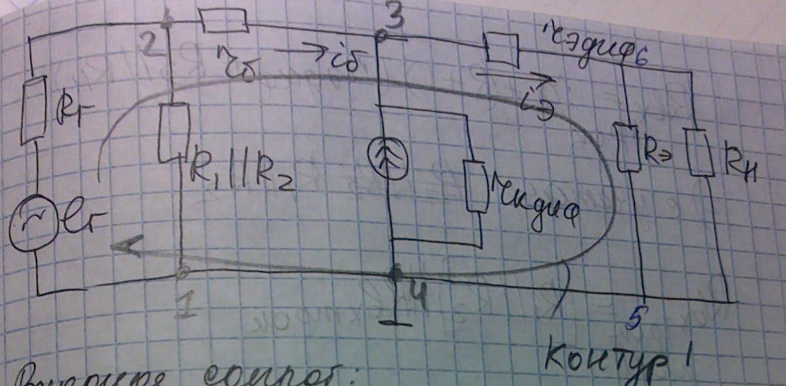
\includegraphics[scale=0.7]{OK1.png}}
\caption{ОК1}
\end{figure}
\end{center}
Важные моменты:
1) Нагрузка цепляется в цепь Э, следовательно 100\% отрицательная связь;
2) Большое входное сопротивление;
3) Малое выходное (хорошее согласование);
4) Не усиливает по напряжению, лучше всех усиливает по току.

1. Входное сопротивление:
$$
R_{вх} = \frac{U_{вх}}{I_{вх}}
$$
$$
U_{вх} = e_{г}-i_{вх}*R_г
$$
1) Без учёта R_{1}//R_{2}:
Контур 1-2 по второму закону Кирхгофа:
$$
U_{вх}=\varphi_{2}-\varphi_{1}=i_{б}*r_{б}+i_{э}*(R_{э}//R_{н}+r_{э_дифф})=i_{б}*(r_{б}+(B+1)*(R_){э}//R_{н}+r_{э_дифф}))
$$
$$
R_{вх}=\frac{U_{вх}}{i_{вх}}=\frac{i_{б}*(r_{б}+(B+1)*(R_){э}//R_{н}+r_{э_дифф}))}{i_{б}}
$$
$$
R_{вх_тр.ок}=r_{б}+(B+1)*(r_{эдифф}+R_{э}//R_{н})
$$
2) С учётом R_{1}//R_{2}:
$$
R_{вх_тр.ок_полн}=[R_{1}//R_{2}]//R_{вх_тр.ок}
$$
2. Выходное сопротивление:
Выходное сопротивление определяется при отключенном напряжении и при нулевом (?) входном сигнале:
$$
R_{вых}=\frac{U_{xx}}{I_{кз}}
$$
$$
U_{xx}=U_{56}(R_{н}=0)
$$
Контур 1: клеммы на нагрузке замкнуты: $ I_{кз}=I_{э} $
$$
U_{56}=U_{R_{1}//R_{2}}+U_{r_{б}}+U_{r_{эдифф}}=[\frac{R_{1}//R_{2}+r_{б}}{B+1}+r_{э}]*i_{э}
$$
$$
R_{\Sigma_56}=[[\frac{R_{1}//R_{2}+r_{б}}{B+1}+r_{э}]//R_{э}]
$$
$$
U_{xx}=R_{\Sigma_56}*i_{э}
$$
$$
R_{вых}=\frac{R_{\Sigma_56}*i_{э}}{i_{э}}=R_{\Sigma_56}=[\frac{R_{1}//R_{2}+r_{б}}{B+1}+r_{э}]//R_{э}
$$
3. Коэффициент передачи по напряжению:
$$
K_{uok}=\frac{U_{вых}}{U_{вх}}=\frac{i_{э}*(R_{э}//R_{н})}{\delta*(R_{вх.тр.ок})}
$$
4. Коэффициент передачи по току:
$$
K_{iok}=\frac{I_{н}}{i_{вх}}
$$
\begin{center}
\begin{figure}[h!]
\center{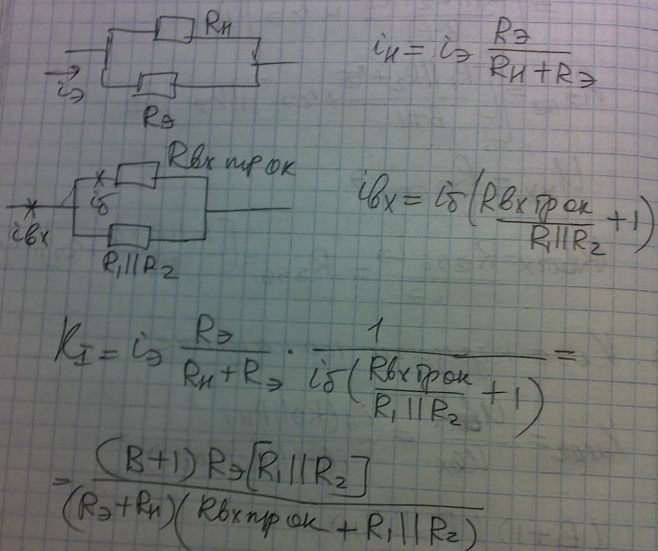
\includegraphics[scale=0.7]{OK2.png}}
\caption{ОК2}
\end{figure}
\end{center}

